\chapter{Theory}\label{sec:theory}

\section{The Standard Model}
The Standard Model (SM) is currently our best theoretical framework for understanding the nature of fundamental particles. 
It is rooted in the idea that particles exist as excitations of quantum fields. These fields are constructed so as to obey 
fundamental symmetries of nature, and they yield the particles of our universe, as well as their interactions. The SM is not only 
elegant and extensive, but provides a wide variety of measurable observables for the experimentalist to probe. So far, many 
measurements have been made of the currently known elementary particles, and the predictions of the SM have held up in each case. In 
this respect, it is a wildly successful theory. In other respects, it is obviously incomplete.

\section{Electroweak Theory}

%\section{Quantum Chromodynamics}

\section{Spontaneous Symmetry Breaking (Higgs Mechanism)}
The electroweak Lagrangian lacking the Higgs term \textcolor{red}{CITE EQUATION} is insufficient. In particular, it does not provide
an explanation for massive gauge bosons. Experimental evidence for massive gauge bosons dates back to the \textcolor{red}{early?}
twentieth century. Beta decay experiments indicated charged current interactions mediated by a massive W boson, and later experiments 
indicated additional neutral current interactions mediated by a massive Z boson (\textcolor{red}{CHECK THIS}). Later in the twentieth 
century (\textcolor{red}{GIVE SPECIFIC DATES/REFS}) the W and Z bosons were discovered. Indeed, the W and Z masses have been found 
to be roughly 80 GeV and 91 GeV respectively. An explanation came in the form of the Higgs mechanism (\textcolor{red}{CITE}),
which spontaneously breaks the SU(2)xU(1) gauge symmetry of the elecroweak Lagrangian. In addition, there arises a real 
Higgs field accompanied by a massive Higgs boson, and fermion masses are explained via their Yukawa couplings to the Higgs boson. 
The discovery of the Higgs boson and the subsequent measurements of its properties have provided proof that the Higgs mechanism 
is indeed a central piece of the Standard Model. 

To understand how the Higgs mechanism works, consider the introduction of a complex scalar field $\sf \Phi$, which 
transforms as a doublet under SU(2).
\begin{equation}
    \label{eqn:higgsField}
    \Phi = 
    \begin{bmatrix}
        \phi^{+} \\ 
        \phi^{0}
    \end{bmatrix}
\end{equation}
Its contribution to the Lagrangian is given by:
\begin{equation}
    \mathcal{L_{H}} = (D^{\mu}\Phi)^{\dagger}(D_{\mu}\Phi) - V(\Phi)
    \label{LHiggs}
\end{equation}
where the Higgs potential takes the form
\begin{equation}
    V(\Phi) = \mu^{2}|\Phi^{\dagger}\Phi| + \lambda \Big(|\Phi^{\dagger}\Phi|\Big)^{2}.
    \label{VHiggs}
\end{equation}
$D_{\mu}$ is the covariant derivative
\begin{equation}
    D_{\mu} = \partial_{\mu} - \frac{ig}{2}\tau\cdot A_{\mu} - \frac{ig'}{2}B_{\mu}Y.
    \label{EWCovariantDeriv}
\end{equation}
Consider the case that the parameters of the Higgs potential $\lambda$ and $\mu$ satisfy the conditions 
$\lambda > 0$ and $\mu^{2} < 0$. Then the shape of the potential is shown in Fig. \ref{fig:VHiggs}. Clearly, there is no minimum of the 
potential at $\Phi = 0$. Rather, an infinite set of minima lie around a circle in the complex plane. Hence, it is said that $\Phi$ 
has a nonzero vacuum expectation value (VEV). The value of the VEV in terms of $\mu$ and $\lambda$ can be determined by explicitly
minimizing the potential:
\begin{align*}
    \frac{\partial}{\partial(\Phi^{\dagger}\Phi)}V(\Phi) &= 0 \\
    \mu^{2} + 2\lambda\Big(|\Phi^{\dagger}\Phi|\Big) &= 0 \\
    \mu^{2} + 2\lambda\Big[(\phi^{+})^{2} + (\phi^{0})^{2}\Big] &= 0 \numberthis
    \label{VHiggsMinimization}
\end{align*}
Clearly, this can be minimized in many ways depending on individual values of $\phi^{+}$ and $\phi^{0}$ in the vacuum. By convention,
and without loss of generality, we choose the case in which $\phi^{+} = 0$. In this case we obtain the equation
\begin{equation}
    \phi^{0} = \sqrt{\frac{-\mu^{2}}{2\lambda}} = \frac{1}{\sqrt{2}}v
\end{equation}
where we have defined $v \equiv \sqrt{-\mu^{2}/\lambda}$.

\begin{figure}
	\begin{center}
	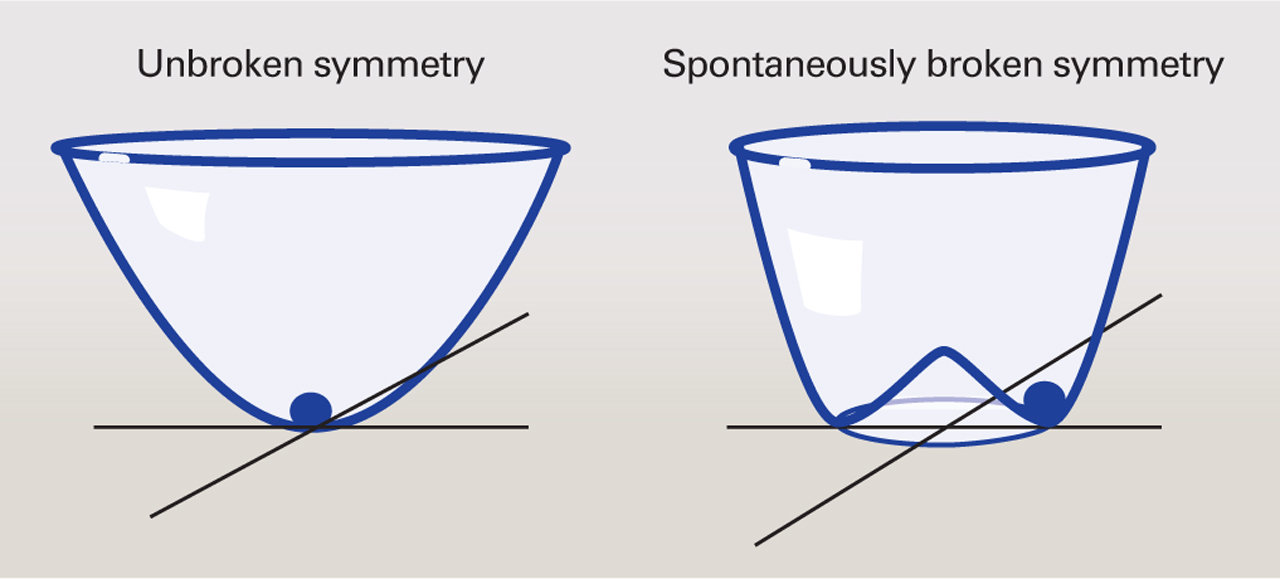
\includegraphics[width=0.75\textwidth]{fig/theory/spont_sym_breaking.jpg}
		\caption{Comparison of the shape of the potential without symmetry breaking and with spontaneous symmetry breaking.}
		\label{fig:VHiggs}
	\end{center}
\end{figure}

The existence of the Higgs VEV has profound implications. To see this, it is helpful to reparameterize the scalar doublet field
$\Phi$ as follows:
\begin{equation}
    \Phi = \frac{1}{\sqrt{2}}e^{i\frac{\tau^{a}}{2}\theta_{a}(x)}
    \begin{bmatrix}
        0 \\
        v + h(x)
    \end{bmatrix}
    \label{reparamHiggsField}
\end{equation}
As $\Phi$ is invariant under local SU(2) gauge transformations, the prefactor may be rotated away. This is equivalent to setting 
$\theta(x) = 0$ in equation \ref{reparamHiggsField}. This choice of gauge is known as the unitary gauge, and leads to 
\begin{equation}
    \Phi = \frac{1}{\sqrt{2}}
    \begin{bmatrix}
        0 \\
        v + h(x)
    \end{bmatrix}
    \label{HiggsFieldUnitaryGauge}
\end{equation}
Given the above form of $\Phi$, we can now evaluate the Higgs Lagrangian (equation \ref{LHiggs}), starting with the kinetic term
$(D^{\mu}\Phi)^{\dagger}(D_{\mu}\Phi)$.
\begin{align*}
    (D^{\mu}\Phi)^{\dagger}(D_{\mu}\Phi) &= \Big| (\partial_{\mu} - \frac{ig}{2}\tau\cdot A_{\mu} - \frac{ig'}{2}B_{\mu}Y)\Phi\Big|^{2} \\
    &= \frac{1}{2}
    \Big| 
    \begin{bmatrix}
        \partial_{\mu} - \frac{i}{2}(gA_{\mu}^{3} + g'B_{\mu}) & -\frac{ig}{2}(A_{\mu}^{1} - iA_{\mu}^{2}) \\
            -\frac{ig}{2}(A_{\mu}^{1} + iA_{\mu}^{2}) & \partial_{\mu} + \frac{i}{2}(gA_{\mu}^{3} - g'B_{\mu})
    \end{bmatrix} 
    \begin{bmatrix}
        0 \\ 
        v + h(x)
    \end{bmatrix} 
    \Big|^{2} \\ &=  
    \frac{1}{2}\Big| 
    \begin{bmatrix}
        -\frac{ig}{2}(A_{\mu}^{1} - iA_{\mu}^{2})(v + h(x)) \\
        \partial_{\mu}h(x) + \frac{i}{2}(gA_{\mu}^{3} - g'B_{\mu})(v + h(x))
    \end{bmatrix}
    \Big|^{2} \\ &= 
    \frac{1}{2}\partial_{\mu}h(x)\partial^{\mu}h(x) + \frac{1}{8}(gA_{\mu}^{3} - g'B_{\mu})(gA^{\mu}_{3} - g'B^{\mu})(v + h(x))^{2} \\ &+ 
    \frac{g^{2}}{8}(A_{\mu}^{1} - iA_{\mu}^{2})(A_{\mu}^{1} + iA_{\mu}^{2})(v + h(x))^{2} \label{kinHiggsExpansion} \numberthis 
\end{align*}
With some foreknowledge of the result, let us define the physical gauge fields and their masses as follows:
\begin{align}
    W_{\mu}^{\pm} &= \frac{1}{\sqrt{2}}(A_{\mu}^{1} \mp iA_{\mu}^{2}) \; &m_{W} = \frac{gv}{2} \\
    Z_{\mu} &= \frac{1}{\sqrt{g^{2} + g'^{2}}}(gA_{\mu}^{3} - g'B_{\mu}) \; &m_{Z} = \sqrt{g^{2} + g'^{2}}\frac{v}{2} \\
    A_{\mu} &= \frac{1}{\sqrt{g^{2} + g'^{2}}}(g'A_{\mu}^{3} + gB_{\mu}) \; &m_{A} = 0
    \label{gaugeBosonsAndMasses}
\end{align}
Then the kinetic term of the Higgs Lagrangian can be recast as
\begin{align*}
    (D^{\mu}\Phi)^{\dagger}(D_{\mu}\Phi) &= \frac{1}{2}\partial_{\mu}h(x)\partial^{\mu}h(x) \\ 
    &+ \frac{1}{2}m_{Z}^{2}Z_{\mu}Z^{\mu} + m_{W}^{2}W_{\mu}^{+}W^{-\mu} \\
    &+ \frac{v}{4}(g^{2} + g'^{2})Z_{\mu}Z^{\mu}h + \frac{1}{8}(g^{2} + g'^{2})Z_{\mu}Z^{\mu}h^{2} \\
    &+ \frac{v}{4}g^{2}W_{\mu}^{+}W^{-\mu}h + \frac{1}{8}g^{2}W_{\mu}^{+}W^{-\mu}h^{2} \label{kinHiggsMasses}\numberthis
\end{align*}
Equation \ref{kinHiggsMasses} provides a great deal of information on the physical ramifications of the Higgs mechanism.
The first term is the kinetic term of the physical Higgs boson field. The second and third terms are the mass terms of the Z and W 
bosons respectively. The fourth and fifth terms show the linear and quadratic couplings of the Z boson to the Higgs boson respectively.
Finally, the sixth and seventh terms show the linear and quadratic couplings of the W boson to the Higgs boson respectively. 
Given the form of equation \ref{HiggsFieldUnitaryGauge}, a similar expansion can be carried out on the Higgs potential
(equation \ref{VHiggs}). Here, the terms involving the physical Higgs boson are most interesting, so constant terms are dropped.
\begin{align*}
    V(\Phi) &= \frac{\mu^{2}}{2}(v+h)^{2} + \frac{\lambda}{4}((v+h)^{2})^{2} \\
    &\rightarrow \lambda v^{2}h^{2} + \lambda vh^{3} + \frac{\lambda}{4}h^{4} \label{expandedVHiggs} \numberthis
\end{align*}
The first term is a Higgs mass term, with $m_{H} = \sqrt{2\lambda v^{2}}$. The second and third terms describe the Higgs 
trilinear and quartic self-coupling respectively.

The Lagrangian including the Higgs doublet $\Phi$ can be further extended to incorporate interactions between the Higgs and fermion fields. These interactions, along with the nonzero Higgs VEV, provide a mechanism to generate the fermion masses. The interactions take the 
form of Yukawa couplings:
\begin{equation}
    \mathcal{L}_{Yukawa} = Y_{ij}^{d}\bar{Q}^{i}_{L}\Phi d_{R}^{j} + Y_{ij}^{u}\bar{Q}^{i}_{L}\tilde{\Phi} u_{R}^{j} 
    + Y_{ij}^{e}\bar{L}^{i}_{L}\Phi e_{R}^{j} + h.c.
    \label{LYukawa}
\end{equation}
where
\begin{equation}
    \tilde{\Phi} \equiv i\tau_{2}\Phi^{*}
    \label{PhiDual}
\end{equation}
Plugging in the unitary gauge $\Phi$ parameterization of equation \ref{HiggsFieldUnitaryGauge}, this evaluates to 
\begin{align}
    \mathcal{L}_{Yukawa} = \frac{Y_{ij}^{d}}{\sqrt{2}}\bar{d}_{L}^{i}(v + h)d_{R}^{j} 
    + \frac{Y_{ij}^{u}}{\sqrt{2}}\bar{u}_{L}^{i}(v+h)u_{R}^{j} + \frac{Y_{ij}^{e}}{\sqrt{2}}\bar{e}_{L}^{i}(v+h)e_{R}^{j}
    \label{expandedLYuk}
\end{align}
It is worth looking closely at the terms in equation \ref{expandedLYuk}. For a given fermion type, the first term in the parentheses
is a fermion mass term. The second term in the parentheses gives the coupling of the fermion to the Higgs boson. With this in mind, 
we observe that the fermion mass is given in terms of the couplings and the Higgs vev by 
\begin{equation}
    m_{f} = \frac{y_{f}v}{\sqrt{2}}
    \label{fermionMass}
\end{equation}
where $y_{f}$ is the relevant value taken from the Yukawa coupling matrix. In addition, we see that the strength of the fermion coupling
to the Higgs boson is given by $\frac{m_{f}}{v}$. Thus, fermions couple to the Higgs boson with strength directly proportional 
to their masses. This result has important consequences in the context of collider experiments, as it regulates the rates of
Higgs production and decay related to each fermion-Higgs vertex. 

%The existence of the Higgs VEV leads naturally to the masses of the W and Z bosons. This can be shown by squaring the covariant 
%derivative acting on the scalar doublet $\Phi$ and evaluating the result in the vacuum. Note that in the vacuum, all terms involving 
%the partial derivative $\partial_{\mu}$ will yield zero contribution. Therefore, keeping only the relevant terms, the squared covariant 
%derivative reduces to
%\begin{equation}
%    |D_{\mu}|^{2} \rightarrow (\frac{g}{2}A_{\mu}^{a}\tau^{a} +\frac{g'}{2}B_{\mu})(\frac{g}{2}A^{b\mu}\tau^{b} + \frac{g'}{2}B^{\mu})
%    \label{covDerivSquared}
%\end{equation}
%Evaluating this in the vacuum yields
%\begin{align}
%    \Delta\mathcal{L} &= \frac{1}{2}
%    \begin{bmatrix}0 & v
%    \end{bmatrix}
%    (\frac{g}{2}A_{\mu}^{a}\tau^{a} +\frac{g'}{2}B_{\mu})(\frac{g}{2}A^{b\mu}\tau^{b} + \frac{g'}{2}B^{\mu}) 
%    \begin{bmatrix}
%        0 \\ 
%        v
%    \end{bmatrix} \\ 
%    \Delta\mathcal{L} &=
%    \frac{1}{2}\frac{v^{2}}{4}[g^{2}(A_{\mu}^{1})^{2} g^{2}(A_{\mu}^{2})^{2} + (g'B_{\mu} - gA_{\mu}^{3})^{2}]
%\end{align}
%From this, we can identify the fields and masses for the positively and negatively charged W bosons and the neutral Z boson and photon. 
%These are as follows:


\section{Higgs Production}

At a hadron collider like the LHC, the Higgs boson can be produced via several different mechanisms, each mechanism occuring at a certain rate. The dominant production 
mechanism is gluon-gluon fusion (ggH), followed by vector boson fusion (VBF) production, which is about an order of magnitude rarer. Less common production mechanisms, but 
still relevant for a search at the LHC, are the associated production mechanisms WH, ZH, and t$\bar{t}$H. The cross sections for each Higgs production mechanism as a function of 
center of mass energy are shown in Fig. \ref{fig:higgs_prod}.

\begin{figure}
	\begin{center}
	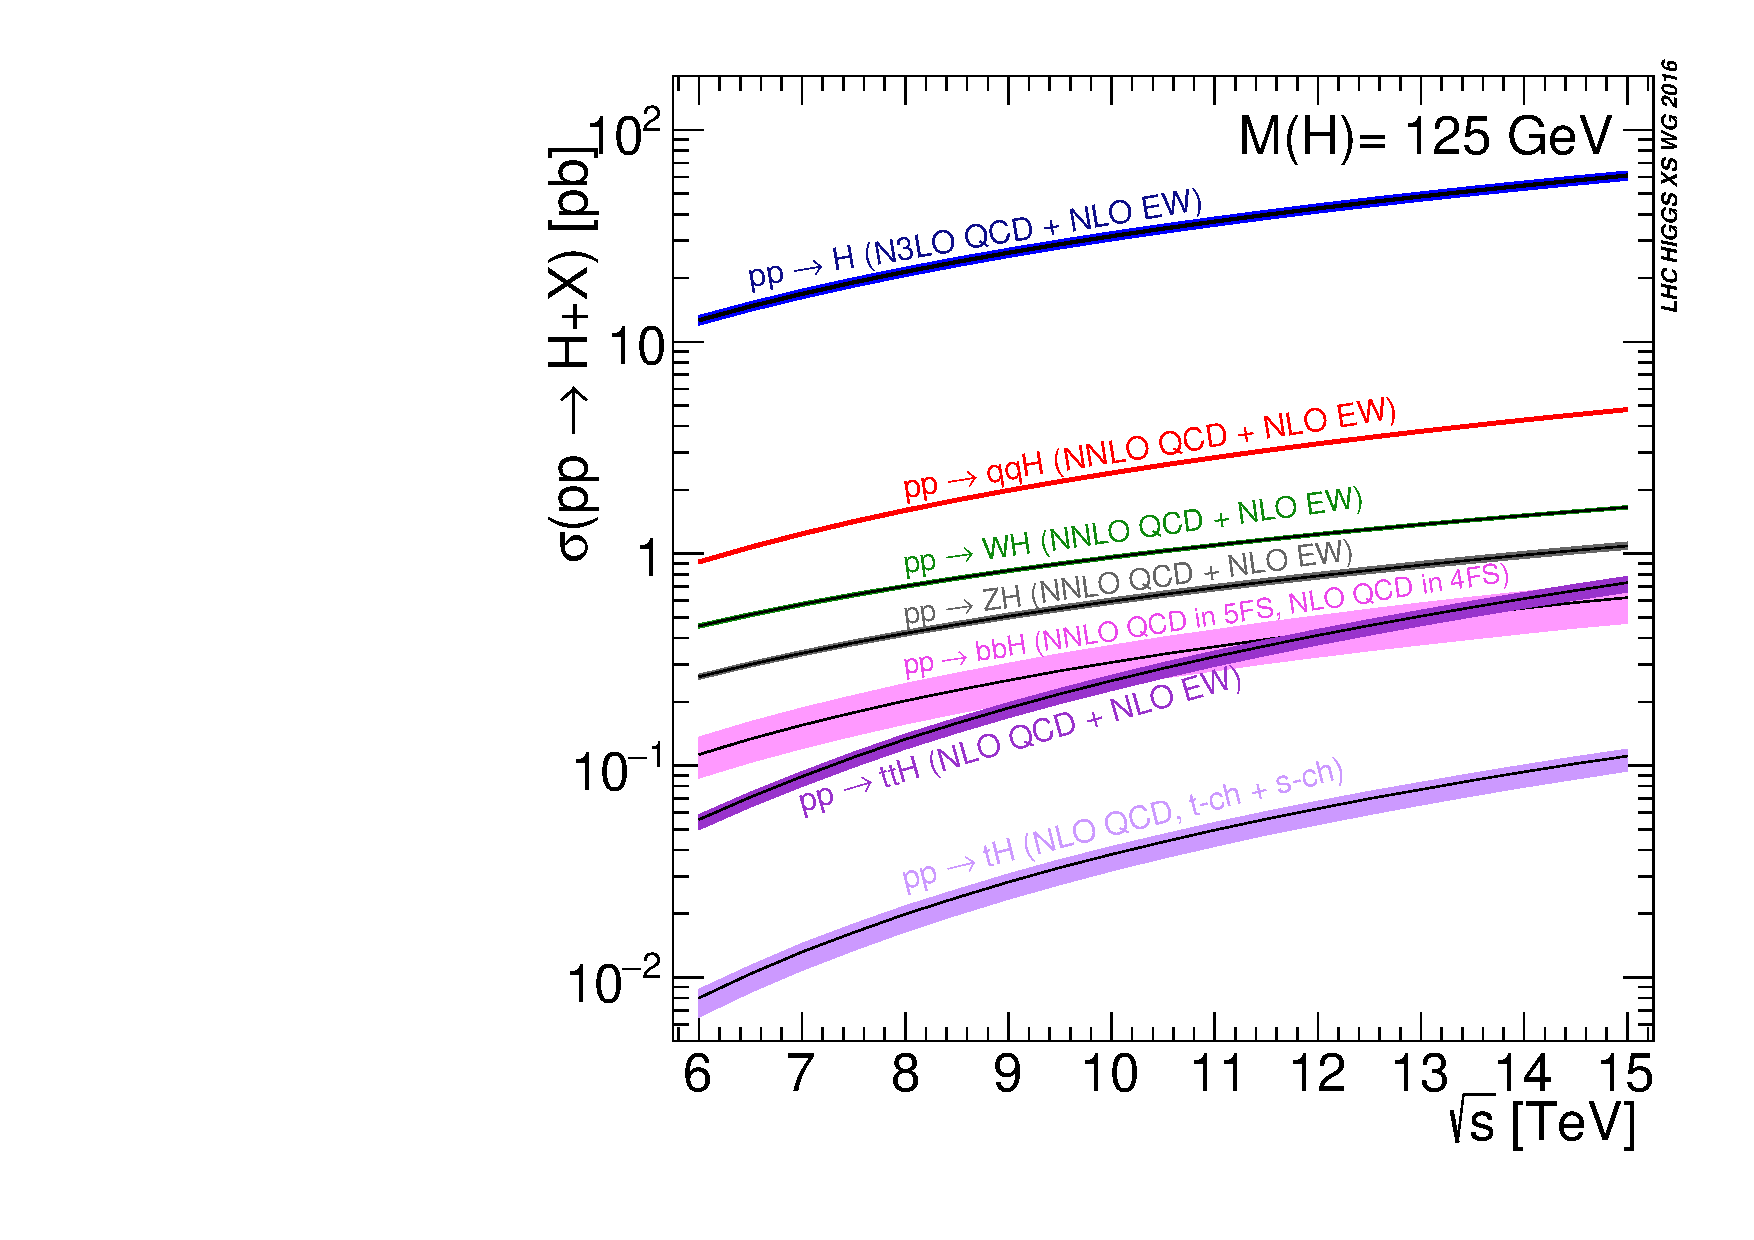
\includegraphics[width=0.75\textwidth]{fig/theory/Plot_Escan_H125_new_sqrt.pdf}
	\caption{Cross sections for different Higgs boson production mechanisms as a function of center of mass energy.}
	\label{fig:higgs_prod}
	\end{center}
\end{figure}

\section{Higgs Decay}

The Higgs boson decays rapidly after it is produced at the LHC. It can decay into a variety of final states, each occuring at a certain rate. Tree-level Higgs decays occur at rates 
proportional to the square of the mass of the decay products. Decays to b$\bar{b}$, WW, $\tau^+\tau^-$, and ZZ, are among the most common and experimentally accessible at the LHC. Other Higgs decays 
occur at loop-level, including $\PH \to \Pg\Pg$ and \hzg. Figure \ref{fig:higgs_br} shows the branching fractions at $\sqrt{s}=13$\TeV for different decay channels as a function of Higgs boson mass. 
We see that the branching fraction of \hzg is suppressed relative to several other production modes, so a search for \hzg must rely on the clean $\ell^+\ell^-\gamma$ signature.

\begin{figure}
	\begin{center}
	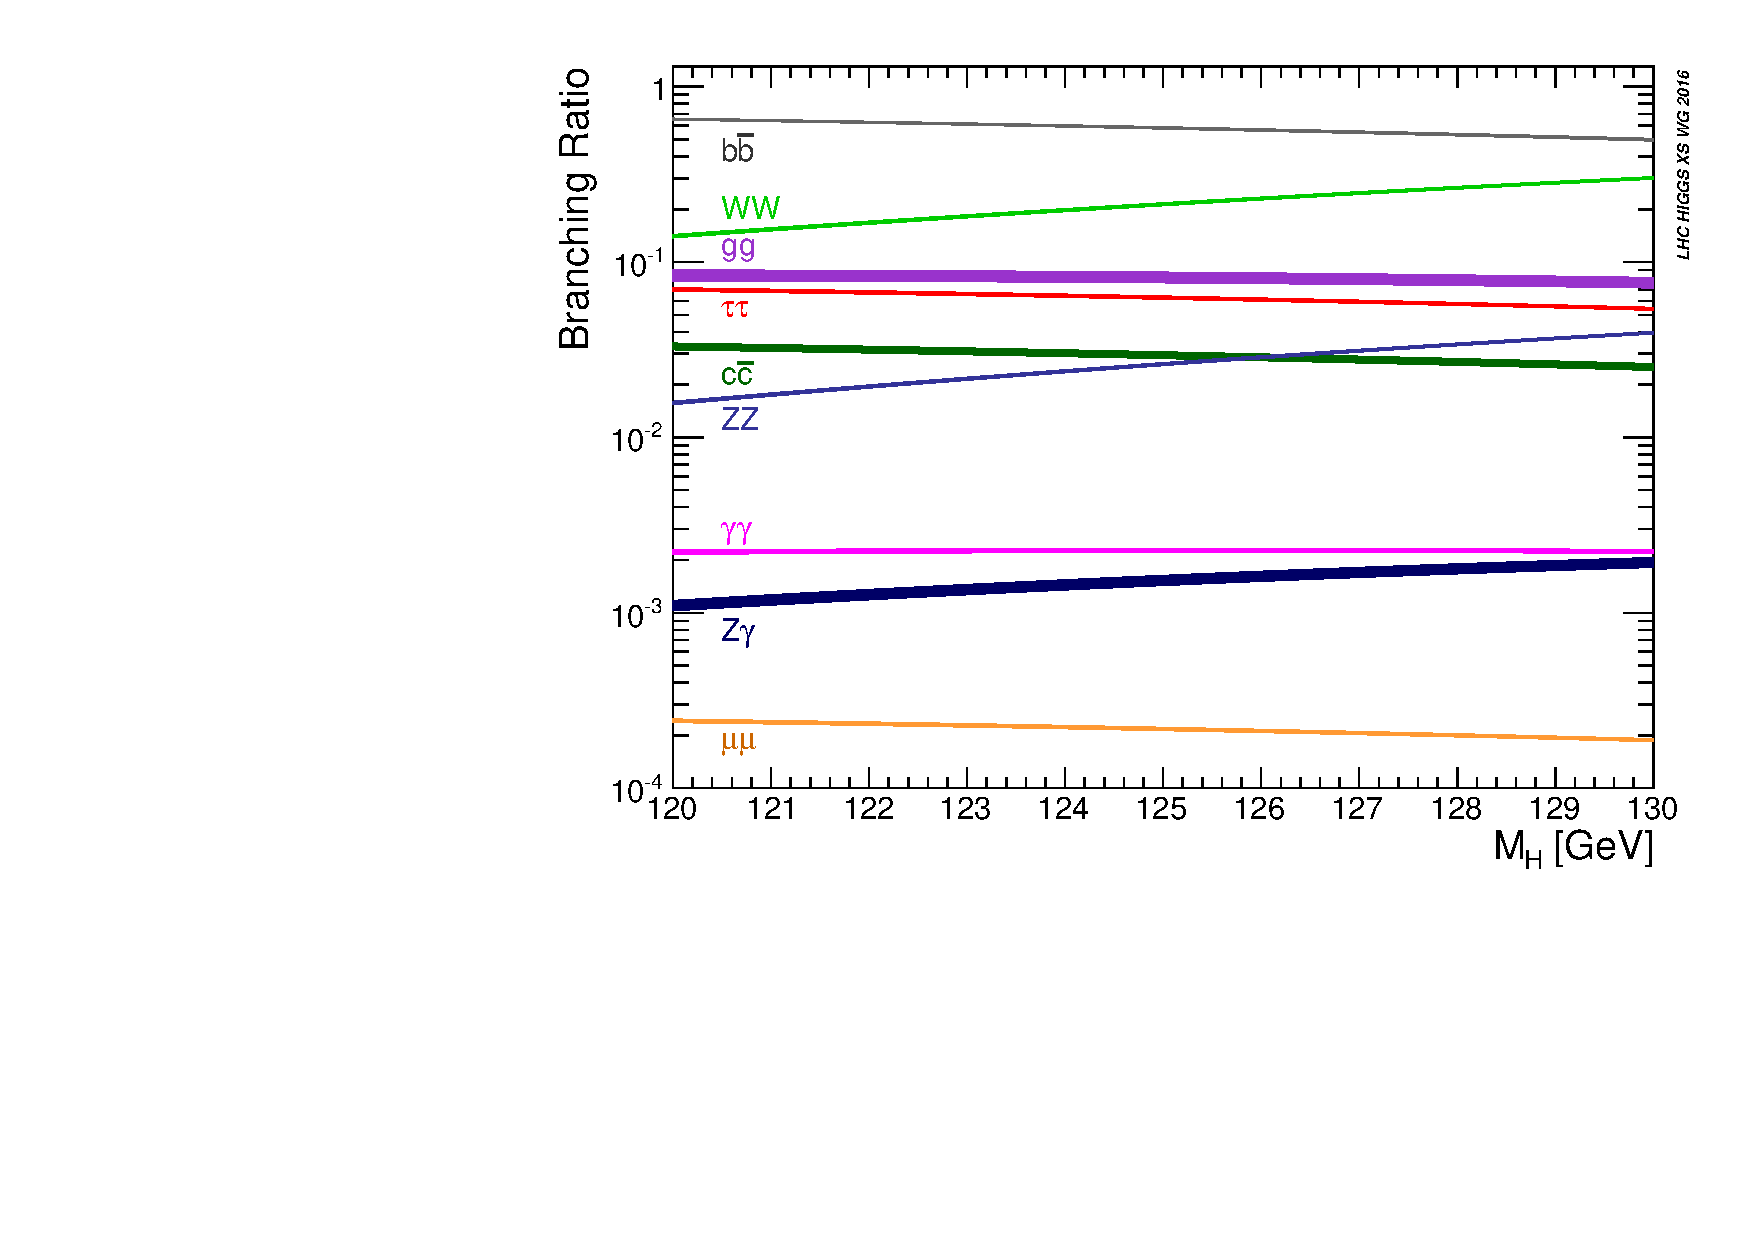
\includegraphics[width=0.75\textwidth]{fig/theory/SMHiggsBR.YR4-rect.pdf}
		\caption{Branching fraction of \hzg decay as a function of Higgs boson mass.}
		\label{fig:higgs_br}
	\end{center}
\end{figure}

\section{Physics Beyond the Standard Model}

